\documentclass[12pt]{article} 
\usepackage{graphicx} % Required for inserting images
\usepackage{amsmath}
\usepackage{subcaption} 
\usepackage[scale=0.8]{geometry}
\usepackage{cite}
\usepackage{caption}

\title{Investigating unconventional superconductivity in the 2D Hubbard-Kanamori model using Functional Renormalization Group (FRG)}
\author{210003218}
\date{February-May 2025}

\begin{document}
\maketitle
\tableofcontents 

\newpage 

\section{Abstract}



Due to its structural resemblance to the high-temperature cuprate superconductors \cite{dagotto1994correlated}, 
the two-dimensional Hubbard model has attracted sustained scientific interest for decades.
This thesis conducts a detailed analysis of the 2D Hubbard model using the truncated-unity functional Renormalisation Group (TU$^2$FRG) method,
within the framework of spin-fluctuation-mediated superconductivity.  The interplay between magenetism and superconductivity is explored 
by systematically varying model parameters such as the on-site Coulomb repulsion, chemical potential, Hund's coupling, next-nearest-neighbor hopping, and the number of orbitals per
site. This approach enables the identification of clear trends in the superconducting critical temperature and order parameter, while also
providing insights into the magnetic ordering. 






\section{Introduction}

Since its discovery in 1911\cite{onnes1911superconductivity}, superconductivity has remained a topic of great scientific interest.
This phenomena, characterised by an abrupt drop in resistance at a so-called "Critical Temperature($T_c$)"\cite{geballe2015tc} is driven by an attractive interaction
between electrons. This attractive interaction gives rise to the formation of electron pairs, famously known as "Cooper pairs"\cite{schrieffer2018theory}. For many 
years after the discovery of superconductivity, physicists
were convinced that BCS-Eliashberg-electron-phonon theory \cite{schrieffer2018theory} provided a complete explanation of the electron pairing mechanism in all superconducting materials. 
However, in 1986, the discovery of the first heavy-fermion superconductor\cite{bednorz1986possible} resulted in the emergence of a whole new class of materials: Unconventional Superconductors. 
These are condensates of cooper pairs formed by a \textbf{different} pairing mechanism than the electron-phonon coupling predicted by BCS theory\cite{hirsch2015superconducting}.
For many materials, there is no consensus on what the mechanism otherwise is. \par 
\medskip

\noindent High-Temperature superconductors are defined by having a critical temperature that exceeds the boiling point 
of Nitrogen (77K). Ever since the discovery of the first high-Tc superconductor\cite{bednorz1986possible}, the search for "(close to-) room temperature" superconductors has been extended to 
all other sorts of unconventional supercondutors. However, a comprehensive understanding of what drives the superconductivity is required in order 
to achieve this. There have been multiple attempts to model the pairing mechanism of some families of high-Tc superconductors, but they have
been greatly limited by the numerical challenges that working with multi-band systems and with spin-orbit coupling (SOC) present. 
This motivates the use of a promising technique: TU$^2$FRG\cite{eckhardt2020truncated,profe2024magic}.\par

\medskip

\noindent Motivated by these challenges and the need for simplified yet insightful models, this work turns to the two-dimensional Hubbard model—one of the most fundamental 
and extensively studied frameworks in condensed matter physics. Functional Renormalisation Group (FRG) is employed to 
investigate the influence of the Coulomb repulsion ($U$) and chemical potential ($\mu$) on the
interplay between magnetism and superconductivity.
This is done under the key assumption that superconductivity arises from spin-fluctuation mediation.
In this work, regions of stable magnetic and superconducting order are identified, and trends in their respective ordering and critical temperatures are presented.
The study is further extended by examining how variations in the next-nearest-neighbor hopping amplitude and the inclusion of a second orbital per site impact all of the above.




\section{Theoretical Background}

\subsection{Unconventional superconductivity}

As previously outlined, unconventional superconductors are those in which the Cooper pair formation is not driven by the convetional electron-phonon coupling. 
This section aims to outline the theoretical background behind a particular class of unconventional superconductors: Spin-fluctuation mediated superconductors. \par
\medskip
\noindent Most generally, the Hamiltonian for a superconducting state can be described as follows:

\begin{equation}\label{General Hamiltonian}
    \hat{H} = \hat{H}^0 + \hat{H}^{cp}
\end{equation}

\noindent where $\hat{H}^{cp}$ describes the pairing interation that leads to the formation of a Cooper pair and is given by:

\begin{equation}\label{Hcp}
    \hat{H}^{cp} = \sum_{k,k'} \Gamma(k, k') c^{\dagger}_{k, \uparrow}  c^{\dagger}_{k', \downarrow} c_{k', \uparrow}c_{-k, \downarrow}
\end{equation}

\noindent For many unconventional superconductors, the form of the effective pairing interaction $\Gamma(k,k')$ has remained as an unanswered question for decades.

\subsubsection{Spin-fluctuation mediated superconductivity}

One emerging theory for some unconventional superconductors such Iron-based or heavy-fermion compounds 
is that the underlying pairing mechanism is driven by spin fluctuations \cite{moriya2000spin}. This section discusses how to
model spin-fluctuation mediated superconductivity for the fluctuation-exchange approximation (FLEX) \cite{esirgen1997fluctuation}. \par
\medskip
\noindent In such cases, the effective pairing interaction $\Gamma(k,k')$ is given by \footnote{Note that this form of pairing interaction 
assumes that the ratio between 
the fluctuation frequence $w_f$ and the Fermi energy is small.}:

\begin{equation}\label{Pairing interaction SF}
    \Gamma(k,k') = \frac{3}{2} U^2 \chi^S(k-k') -\frac{1}{2}U^2 \chi^C(k-k') + U
\end{equation} 

\noindent This equation is taken from Ref.\cite{migdal1958interaction}. Here, U is the on-site Coulumb repulsion and $\chi^S$, $\chi^C$ are the interacting spin-susceptibilities in the Charge (C) and Spin(S) channel respectively. Their form is given below.

\begin{equation}
    \chi^S(q) = \frac{\chi^0(q)}{1 - U \chi^0 (q)}
\end{equation}

\begin{equation}
    \chi^C(q) = \frac{\chi^0(q)}{1 + U \chi^0 (q)}
\end{equation}

\noindent These interacting spin susceptibilities are expressed in terms of the non-interacting dynamic spin susceptibility ($\chi_{ps}^0$) which is stated below without formal proof \cite{moriya2000spin}. 

\begin{equation}\label{chi 0}
    \chi_{ps}^0(q, i \omega) = -\sum_{k} \int_{0}^{\beta} d\tau G^0_{ps}(k+q \tau) G^0_{sp}(k, -\tau)e^{i\omega \tau}
\end{equation} 

\noindent The calculations presented in this project are carried out in the spin-fluctuation framework. 
Whilst this theory has managed to succesfully capture key features in phase diagrams of unconvential superconductors, it also has its limitations.
The most relevant example is that of the cuprate phase diagram.
Spin-fluctuation theory is able to capture the superconducting dome and the correct order parameter \cite{moriya2006developments, scalapino1995case} 
but fails
to describe the characteristic pseudo-gap\cite{timusk1999pseudogap}. 

\subsection{Hubbard-Kanamori Model}

\subsubsection{Tight Binding Models}

The Tight Binding Model is a central element of condensed matter physics \eqref{TBM}. In this model, electrons are bound in orbitals (called sites) around the lattice ions.
Due to the overlap between the quantum mechanical wavefunctions that describe these sites, electrons are allowed to 'hop' to neighbouring sites. The probability that this hopping process will occur is given by a tunnelling amplitude, which can be calculated using a hopping integral. \par
\medskip
\noindent This work is carried out in the tight-binding model framework, where the magnitude of the tunnelling amplitudes is at first treated as a free parameter. 
The starting point is a simple nearest-neighbour hoppping tight binding model. 
The effect of introducing a next-nearest-neighbour hopping and an extra orbital per site
is then investigated \textit{(See Fig. \ref{fig:2D Hubbard model})}.



\begin{equation} \label{TBM}
    \hat{H}_{TB}(\b{R}) = \sum_{ij\sigma} t_{ij}(\hat{c}_{i\sigma}^{\dagger}\hat{c}_{j \sigma} + h.c)
\end{equation}


\begin{figure}[htbp]  % Placement: Here, Top, Bottom, Page
    \centering
    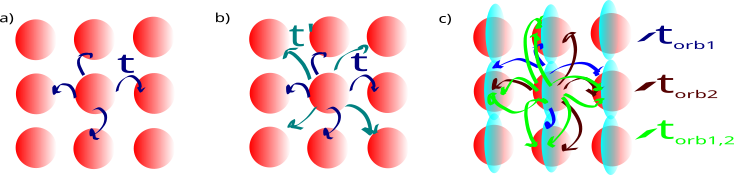
\includegraphics[width=0.9\textwidth]{2Dhubbardmodel.png}  % Adjust width as needed
    \caption{\textbf{Two-Dimensional Tight-Binding Models:} Three pannels showing the tight binding models for the 1NN, 1NNN and 1NN2 models discussed in Section~\ref{subsec:1NNModel},~\ref{subsec:1NNNModel} and~\ref{subsec:1NN2Model} respectively. Fig a) shows the Nearest-neighbour hopping case, where \textit{t} depicts the hopping amplitude between the neighbouring sites. Fig b) shows the inclusion of the next-nearest neighbour hopping- magnitude given by \textit{t'}.
    Fig c) Shows the extension to the two-orbital case, depicting  same orbital ($t_{orb1}$, $t_{orb2}$) and different orbital ($t_{orb1,2}$) nearest-neighbour hopping. Note that this is just a pictorial representation of the orbitals, and that it does not correspond to a particular choice of orbitals or their real space projection. }
    \label{fig:2D Hubbard model}
\end{figure}

\newpage

\subsubsection{Hubbard Model}
\label{subsec: HubbardModel}

The  tight binding model as defined above fails to account for any interactions between neighbouring electrons. This motivates the extension of this model to the Hubbard model \eqref{t Hubbard model}, which includes the (onsite) Coulomb repulsion between electrons. Despite its simple form, this model can describe very rich physical phenomena.
In particular, it becomes very interesting to study when U and t are of comparable order, since it highlights the competing phenomena that take place in correlated systems. 
The 2D Hubbard model remains unsolved to date, but is able to predict all sorts of correlated phases: it describes metals, insulators, superconductors and other exotic phases\cite{white1989numerical,hirsch1985two, anderson1990luttinger,sun2011nearly}. 
This model has been widely studied since it resembles the structure of the cuprate high-temperature superconductors \cite{dagotto1994correlated}. 




\begin{equation}\label{t Hubbard model}
    \hat{H} = \sum_{ij\sigma} -t_{ij}(\hat{c}_{i\sigma}^{\dagger}\hat{c}_{j \sigma} + h.c) 
    + U \sum_{i} \hat{n}_{i \uparrow} \hat{n}_{i \downarrow}
\end{equation}





\subsubsection{Hubbard-Kanamori Model}
\label{subsubsec: HKmodel}
In the case of materials with a multi-band and/or multi-orbital nature, the Hubbard model is not sufficient to capture all of the physical phenomena. This motivates the extension of the Hubbard Model to the Hubbard-Kanamori model\cite{sherman2020hubbard} by including a Hund's coupling term.

\begin{equation} \label{Hubbard-Kanamori Model}
    H_{int} = U \sum_{is}n_{i,s\uparrow}n_{i,s\downarrow} + \frac{V}{2} \sum_{i,s,t \neq s} n_{is}n_{it} -\frac{J}{2} \sum_{i,s,t \neq s} \vec{S}_{is} \cdot \vec{S}_{it} 
    + \frac{J'}{2} \sum_{i,s,t \neq s} \sum_{\sigma} c_{is\sigma}^{\dagger}c_{is\bar{\sigma}}^{\dagger}c_{it\bar{\sigma}}c_{it\sigma}
\end{equation}

\noindent Here, $U$ and $V$ represent the electronic interactions in the same and different orbitals respectively. For generality, the intraorbital exchange $J$ and the 'pair hopping' term $J'$ following from Hund's rule coupling have been separated.  
Note that this Hamiltonian is relevant for the later section of this project, where the model is extended to a two-orbital, two-dimensional Hubbard Model.

\subsection{Theoretical Background in FRG}

Solving the Hubbard-Kanamori Hamiltonian is rather challenging, which is why we resort to numerical techniques such as FRG to do so. FRG falls into the category of many other weak-coupling techniques (such as Mean field-theory\cite{kadanoff2009more}, pertubation theory\cite{nagaosa2013quantum}, Density Functional theory\cite{kohn1965self} or Random Phase approximation\cite{bohm1951collective}).
In these theories, interactions between electrons are considered to be weak. This allows one to effectively model the electrons in the system as free particles 
and treat their interactions as a pertubation. In the non-interacting limit, the method is therefore exact. Beyond this limit, the precision of the method is controlled by the ratio between the interaction
strength and the bandwidth of the system. 

\medskip

\noindent In this section the theoretical framework in which FRG calculations are performed is outlined. The central element of FRG is a flow equation that describes the evolution of the effective action of the system with respect to a scalar/flow parameter Lambda $\Lambda$ \textit{(See section ~\ref{subsubsec:Flow Equation})}.
The flow equation can be solved exactly for a limited number of systems, so for most scenarios an approximation has to be made in order to reach a solution in a reasonable computational time. 
More details of how this approximation is performed and the limitations it presents can be found in Section~\ref{subsubsec:Truncation scheme}. For the systems explored in this project only two-particle
interactions are considered and any higher order terms are neglected.
This allows for the effective action of the system to be separated into three terms, which correspond to three physical channels: Superconductivity, Spin-Density and Charge-Density Waves.
The calculation is then performed to determine the "winning channel" which will correspond to the respective physical phase that the model exhibits. This rather "hand-wavy" overview of FRG is represented in a flowchart below \textit{ (See Fig.\ref{fig:FRGflowdiagram})}.
For a more rigorous explanation the reader is referred to the sections below. 

\begin{figure}[htbp]  % Placement: Here, Top, Bottom, Page
    \centering
    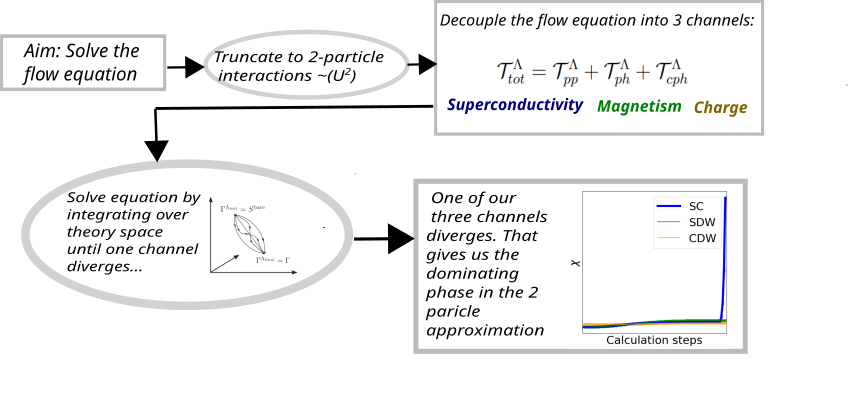
\includegraphics[width=0.9\textwidth]{FRGflowdiagram.png}  % Adjust width as needed
    \caption{\textbf{FRG Flowchart:} Schematic diagram outlining the TU$^2$FRG calculation steps. Starting from the flow equation and applying the truncation scheme in order to decouple the action into three "physical" terms. 
    The flow equation can then be solved by calculating each channel separatedly and taking the dominating phase to be the channel that diverges.}
    \label{fig:FRGflowdiagram}
\end{figure}

\subsubsection{Flow equation}
\label{subsubsec:Flow Equation}

In this section the derivation of the flow equation is outlined. For such, it is assumed that the reader has grasped a strong understanding in Quantum Field theory and many-body physics.
If interested in the finer details of the derivation, the reader is refferred to \cite{metzner2012functional}. \par
\medskip
\noindent The central elements of statitiscal physics are the partition function, the canonical potential and its Legendre transformations. 
These are such powerful physical quantities that one can derive all physical observables from them.
For quantum many-body problems, one works instead with partition functional, defined as follows in Eq.\ref{partition functional}:

\begin{equation}\label{partition functional}
    \mathcal{Z}[\bar{\eta}, \eta] = \int \mathcal{D} \bar{\psi} \mathcal{D}\psi e^{\mathcal{S}[\bar{\psi}, \psi]}e^{(\bar{\eta}, \psi)+(\eta, \bar{\psi})}
\end{equation}

\noindent In the case of fermionic systems, the action in the exponent of Eq.\ref{partition functional} takes the form shown below.
\begin{equation} \label{action}
    \mathcal{S}[\psi, \bar{\psi}] = -(\bar{\psi}, G_0^{-1} \psi) + V[\psi, \bar{\psi}]
\end{equation}

\noindent Here, $V[\psi, \bar{\psi}]$ is an arbitrary many-body interaction and $G_0$ represents the propagator of the non-interacting system. This equation contains the shorthand notation $(...)$, which represents the sum $\sum_x \bar{\psi}(x)(G_0^{-1}\psi)(x), (G_0^{-1}\psi)(x) = \sum_{x’}G_0^{-1}(x,x’)\psi(x’)$. In this sum, the Grassman field index $x$ represents all the quantum numbers of the single-particle basis and imaginary time.\par
\medskip

\noindent Note that in the limiting case where $V=0$, the path integral in Eq.\ref{partition functional} is exactly solveable. 
However, the situation becomes considerably more intricate when electronic correlations are taken into account.
The main idea behind FRG is to introduce a cut-off in the non interacting Green's function ($G_0 \rightarrow G_0^{\lambda} = f(\lambda)G_0$). 
This cutoff is then interpolated between the solveable intital state and the full path integral solution by susbsequently including electronic interactions. For a spin-independant system this would transform the 
bare propagator as shown in Equations (\ref{propagator transform 1}) and (\ref{propagator transform 2}). 

\begin{equation} \label{propagator transform 1}
    G_0(k_0, \textbf{k}) \rightarrow G_0^{\lambda}(k_0, \textbf{k})
\end{equation}


\begin{equation} \label{propagator transform 2}
    \frac{1}{ik_0 - \xi_{\textbf{k}}} \rightarrow \frac{\theta^{\textbf{k}}}{ik_0 - \xi_{\textbf{k}}}
\end{equation}

\noindent where $\theta^{\lambda}(\textbf{k})$ is defined, for example, as follows:

\begin{equation} \label{theta def}
    \theta^{\lambda}(\textbf{k}) = \Theta(|\xi_{\textbf{k}}| - \lambda)    
\end{equation}

\noindent With this particular choice of cutoff scheme, the calculation then excludes points close to the Fermi Surface \textit{(See Fig.\ref{fig:Truncation})}. \par
\begin{figure}[htbp]  % Placement: Here, Top, Bottom, Page
    \centering
    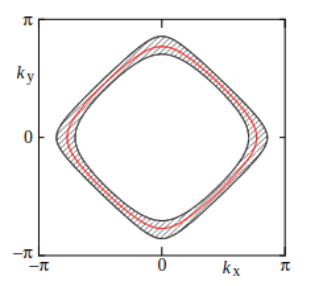
\includegraphics[width=0.35\textwidth]{Truncation.png}  % Adjust width as needed
    \caption{\textbf{Cut-off scheme example:} Momentum space region(shaded in grey) around the Fermi-surface(red) that is excluded 
    by a momentum cut-off for a 2D square lattice with a lattice constant of 1\AA. Taken from \cite {metzner2012functional}}.
    \label{fig:Truncation}
\end{figure}

\medskip
\noindent In the following steps the derivation will proceed in the framework of the  so-called "effective action" ($\mathcal{T}[\psi, \bar{\psi}]$).
This is the Legendre transformation of the Greens function functional ($\mathcal{G}[\eta, \bar{\eta}]$), defined below in Equations (\ref{Greens function functional}, \ref{G term in effective action}) and (\ref{Effective action}) respectively. 
\textit{(For reasons that
are beyond the scope of this project it is more convinient to work with the effective action than it is to do so with the partition functional.) \footnote{If interested in why see Ref. \cite{metzner2012functional}}}

\begin{equation} \label{Greens function functional}
    \mathcal{G}[\eta, \bar{\eta}] = -ln(\mathcal{Z}[\eta, \bar{\eta}])
\end{equation}

\begin{equation}\label{G term in effective action}
    \mathcal{G}[\eta, \bar{\eta}] = 
    -ln \int{\mathcal{D}\psi \mathcal{D} \bar{\psi}e^{-\mathcal{S}[\psi, \bar{\psi}]}e^{(\bar{\eta}, \psi) +(\bar{\psi}, \eta)}}
\end{equation}

\begin{equation} \label{Effective action}
    \mathcal{T}[\psi, \bar{\psi}] = (\bar{\eta},\psi) + (\bar{\psi},\eta) + \mathcal{G}[\eta, \bar{\eta}]
\end{equation}


\noindent The next step is to introduce a scalar flow parameter $\lambda$ into the generating functionals defined above. This is done in the same manner as is outlined in the example shown in Equations \ref{propagator transform 1} $\&$ \ref{propagator transform 2}. 
But more generally, has to be performed such that the generators recover their orginal structure at $\lambda = 0 $.
After a series of algebraic manipulations, which are ommitted here but can be found in \cite{metzner2012functional}, one arrives at the exact functional flow equation for the effective action:


\begin{equation} \label{eq:ExactFunctionalFlowEquation}
    \frac{d}{d\Lambda} \mathcal{T}^{\Lambda}[\psi, \bar{\psi}] = (\bar{\psi}, \dot{Q}_0^{\Lambda} \psi) - \frac{1}{2} \text{tr} \big( \dot{Q}_0^{\Lambda} (\boldsymbol{\Gamma}^{(2)\Lambda}[\psi, \bar{\psi}])^{-1} \big).
\end{equation}

\noindent Where $\Gamma^{(2)\lambda}[\psi, \bar{\psi}]$ and  $\b{Q}_0^{\Lambda}$ are given by equations (\ref{Gamma term}) and (\ref{Q0 term }) respectively.



\begin{equation}\label{Gamma term}
\Gamma^{(2)\lambda}[\psi, \bar{\psi}] = 
\begin{bmatrix}
\bar{\delta} \delta \Gamma[\psi, \bar{\psi}](x',x) & \bar{\delta} \bar{\delta} \Gamma[\psi, \bar{\psi}](x',x) \\
\delta \delta \Gamma[\psi, \bar{\psi}](x',x)  & \delta \bar{\delta} \Gamma[\psi, \bar{\psi}](x',x)
\end{bmatrix}
\end{equation}



\begin{equation}\label{Q0 term }
\b{Q}_0^{\Lambda} =
\begin{bmatrix}
Q_0^{\Lambda} & 0 \\
0 & -Q_0^{\Lambda t}
\end{bmatrix}
= diag(Q_0^{\Lambda}, - Q_0^{\Lambda t}),
\end{equation}

\noindent This flow equation is the central element of FRG and the sections below outline how to solve it.


\subsubsection{Truncation scheme (TU$^2$FRG)}
\label{subsubsec:Truncation scheme}


The flow equation derived above can be solved exactly only for a small class of systems; for most models, Functional Renormalisation Group (FRG) 
calculations are highly computationally expensive.
In order to tackle this issue, the truncated unity approximation (TU$^2$FRG) was introduced in 2020\cite{eckhardt2020truncated}. 
The main idea behind this scheme is to find a new basis that, with a controlled loss of accuracy, can represent all 
of the required elements in a compressed way. It can be shown\cite{lichtenstein2018functional}, that such a basis can be constructed and is 
well defined in the case where the calculation is constrained to terms in the order of U$^{2}$ \textit{(two-particle interactions)}.
Partitions of unity \footnote{A detailed explanation of what these are can be found in \cite{lichtenstein2018functional}} are then introduced into a specific part of the flow equation. This reduces an otherwise computationally expensive nested integral to a matrix product. 
Details of how this truncation is incorporated are ommitted but the reader is referred to Appendix. (REFERENCE appendix).\par
\medskip

\noindent Whilst the truncated scheme presents advantages in computational efficiency, particularly for models with broken translational symmetry, it also has its limitations. 
TU$^2$FRG relies on short-range interactions, thus struggling to capture strongly correlated phases. 
This is particularly relevant for the study of the 2D Hubbard model. TU$^2$FRG will not be able to capture
the characteristic Mott insulating phase of the Cuprate phase diagrams\cite{imada1998metal}, which limits how well the results presented in this project can be directly compared with existing literature. 
More importantly, the truncation scheme has a direct consquence on the accuracy of the predicted phase transition temperature ($T_c$). Whilst it is able to correctly capture
the trends in $T_c$, the values predicted are much higher than what is reasonable to expect in real materials.
Nevertheless, TU$^2$FRG successfully captures the competition between Magnetic and Superconducting instabilities, a central focus of the results presented in this project. 
\subsubsection{Decoupling of flow equation}
After constraining ourselves to the case of two-particle interactions in the framework of translationally invariant systems, one can decouple the two-particle coupling as a function of the flow parameter $\lambda$ into three channels:

\begin{equation} \label{V decoupling}
    V(k1,k2,k3)= V_{k_1, k_2, k_3}^{(0)} - \phi^{P}_{k_1 +k_2, \frac{k_1 - k_2}{2}, \frac{k_4-k_3}{2}} + \phi^{C}_{k_1 - k_3, \frac{k_1 +k_3}{2}, \frac{k_2+k_4}{2}} +\phi^{D}_{k_3- k_2, \frac{k_1 + k_4}{2}, \frac{k_2+k_3}{2}}
\end{equation}

\noindent Here, the three channels correspond to a particle-particle, crossed particle-hole and (three) direct particle-hole terms given explicitly below in terms of the respective effective actions. They represent all possible ways in which the two particle interactions can occur in the correlated system. The particle-particle (P), cross-particle-hole (C) and direct-particle-hole (D) channels
correspond to the Superconducting, Charge and Magnetic phases respectively. 

\begin{equation}
    \dot{\phi}^{P}_{k_1 +k_2, \frac{k_1 - k_2}{2}, \frac{k_4-k_3}{2}} = - \mathcal{T}_{pp}(k1,k2,k3)
\end{equation}


\begin{equation}
    \dot{\phi}^{C}_{k_1 - k_3, \frac{k_1 +k_3}{2}, \frac{k_2+k_4}{2}} = - \mathcal{T}_{cr-ph}(k1,k2,k3)
\end{equation}

\begin{equation}
    \dot{\phi}^{D}_{k_3- k_2, \frac{k_1 + k_4}{2}, \frac{k_2+k_3}{2}} = - \mathcal{T}_{d-ph}(k1,k2,k3)
\end{equation}

\noindent This enables the effective action to be treated as a separable object:

\begin{equation}
    \mathcal{T}[\psi, \bar{\psi}] = \mathcal{T}_{pp}[\psi, \bar{\psi}] + \mathcal{T}_{ph}[\psi, \bar{\psi}] + \mathcal{T}_{cph}[\psi, \bar{\psi}]
\end{equation}

\medskip





\subsubsection{Instability calculation}

This section outlines the procedure that follows after decoupling the effective action and flow equation. For more details the reader is refferred to\cite{profe2023functional}. 
An FRG calculation on the decoupled action yields the self-energy and the two-particle vertex\footnote{For precise definitions of these quantities, see \cite{metzner2012functional}}.
Although these quantities are not directly measurable, they serve as the foundation for further analysis. The first post-processing step involves
identifying which of the three interaction channels diverges, revealing the leading susceptibility. Mean-field analysis is then performed at the critical scale to determine the ordering symmetry 
and derive a linearized gap equation. This, in turn, enables the computation of 
the superconducting gap and order parameter.


\section{Computational Methods}

This section outlines how the concepts presented above link together and are implemented for the purpose of this project. 
The general aim is to solve the 2D Hubbard-(Kanamori) model. This is achieved computationally, using the divERGe package \textit{(See section ~\ref{subsec:diverge})} which implements the TU$^2$FRG
formalism discussed in Section \ref{subsubsec:Truncation scheme}. All of the calculations are carried out under the assumption that the superconductivity 
is spin-fluctuation mediated. This section outlines the methods followed to calculate the required Tight-Binding Models for each of the systems, the utilisation of 
Diverge to solve them and some of the required convergence techniques. 

\subsection{Tight-Binding Models}

\label{subsec:TBM1NN2}

This project discusses three models: the 1NN, 1NNN and 1NN2 model (\textit{See Fig.\ref{fig:2D Hubbard model}}). For the first two, the hopping parameters in the tight-binding model are treated as free parameters. 
For the later, the hopping parameters are determined using the method described below. \par
\medskip
\noindent Constrained to the case of a single layer, the 1NN model is extended to a multi-orbital system by
including two-orbitals per site and investigating the effect of the interorbital hopping. To allow for future comparison with
existing literature\cite{sakakibara2024possible}, a $d_{x^2-y^2}$ and $d_{3z^2 -r^2}$ orbital are included. 
Their respective hopping parameters are determined using the  table of interatomic matrix elements calculated by J.C. Slater and G.F. Koster\cite{slater1954simplified}. 
In this calculation, the values of the $\sigma,  \pi, \delta$ bond strength  are approximated to  $\approx  1, 0.5, 0.05eV$ respectively in order to capture their relative values\cite{blanksby2003bond, mcgrady2015introduction, krapp2008strength}.
A table summarising the estimated parameters for the models  discussed in Section~\ref{subsec:1NN2Model} is shown below.

\begin{table}[h]
    \centering
    \begin{tabular}{|c|c|c|c|c|c|}
        \hline
       Model &$t^{[1,0,0]}_{3z^2-r^2}$  &$t^{[0,1,0]}_{3z^2-r^2}$  &  $t_{x^2 - y^2}$ &  $t^{[1,0,0]}_{x^2 - y^2 -3z^2-r^2} $ & $t^{[0,1,0]}_{x^2 - y^2 -3z^2-r^2} $ \\
        \hline
        & -0.781 & -0.719  &  -0.375 & -0.402 & -0.310\\
        \hline
        1NN2MN & on &  on  & on  & off & off  \\
        \hline
        1NN2MY & on &  on  & on  & on & on \\
          
        \hline
    \end{tabular}
    \caption{\textbf{Nearest neighbour hopping parameters for 2D  two-orbital Hubbard models.} First row shows the calculated hopping parameters.
    These are labelled by a lower and upper index reresenting the orbital and the direction of hoping respectively.
    Other rows in the table show which hopping parameters were included in each of the two models from Section \ref{subsec:1NN2Model}.}
    \label{tab:2D2orbparams }
\end{table}

\subsection{divERGe}
\label{subsec:diverge}

divERGe is an open-source, high-performance, C/C++/Python library that includes a truncated unity FRG (TU$^2$FRG) computational backend\cite{profe2024diverge}. 
At the core of the truncated-unity calculation is a model that incorporates all the essential physical parameters. This model must accurately reflect the system's kinematics, based on its real-space hopping parameters.
It is equally important to define structural details such as the Bravais lattice vectors, the number of atoms per unit cell, 
and the number of orbitals per atom. Once the model is established, six input parameters must be specified for the calculation to proceed: 
the strengths of the Coulomb repulsion ($U$) and Hund’s coupling ($J$), the value of the chemical potential ($\mu$), as well as the form factor, nk and nkf
values. The latter three are discussed in more detail in Section \ref{subsec:convergence}.\par
\medskip
\noindent With the model constructed and all necessary parameters defined, 
the calculation can proceed. Under the approximations described in Section \ref{subsubsec:Truncation scheme},
the flow equations are integrated numerically from high energy scales ($\lambda = \infty$) down to low scales ($\lambda = 0$), 
by incrementally stepping from $\lambda$ to $\lambda + d\lambda$. This integration continues until a phase transition is detected—signaled 
by the divergence of one of the interaction channels—or until a minimum value of $\lambda$ is reached. In the latter case, the system is considered to remain 
in a Fermi-liquid state. All such computations were performed on the high-performance computing (HPC) cluster at the University of St Andrews.


 

\subsection{Convergence of Calculation}
\label{subsec:convergence}
In the truncated-unity approximation, several convergence tests must be performed to ensure the accuracy of the calculations.
These tests include checking the form factor convergence and the number of k points.

\subsubsection{Form factor convergence}

The set of orthogonal basis functions ($f_m$) used to describe the Truncated space\textit{(See section \ref{subsubsec:Truncation scheme})}
in momentum representation is called the \textbf{form factors}. In the case of the square lattice, 
these take the form of delta functions in real space. The form factors are arranged as circles with increasing radii around the origin. This effectively leads to a "bond-like" representation where the form-factor number
essentially determines how many of the neighbouring bonds are accounted for in a calculation for each point. For mathematical rigour on the definition of the form factor, the reader is referred to \cite{lichtenstein2018functional}. \par

\medskip


\noindent The divERGe package allows the user to modify the number of form-factor shells accordingly. Choosing an appropraite values ultimately comes down to a trade 
between computational accuracy and expensiveness. 
For the results in this project, the form factor value was set at 4\AA\footnote{This is equivalent to a number of form factor shells of 4 since the lattice spacing of the models here is set to 1\AA.} after the convergence of the 
the calculations was tested accordingly for a range of points in the phase diagram \textit{(an example of such tests is shown in Fig.\ref{fig:Formfactorconvergence} )}. Moreover, this is in agreement with values used in previous literature\cite{lichtenstein2018functional}. 

\begin{figure}[htbp]  % Placement: Here, Top, Bottom, Page
    \centering
    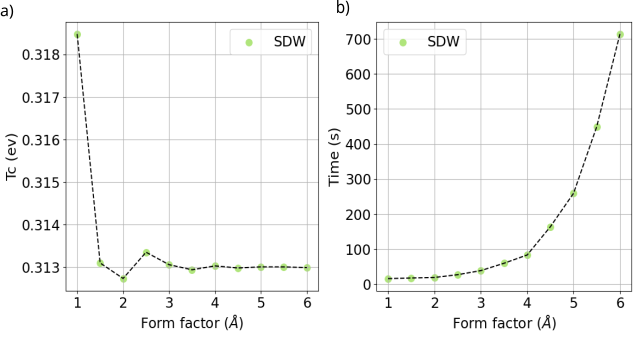
\includegraphics[width=0.6\textwidth]{convergence.png}  % Adjust width as needed
    \caption{\textbf{Convergence testing:} Fig a) Transition temperature as a function of form factor for the 1NN model, U = 5.00, $\mu$ = 0.20eV. Fig b) Time taken for calculation
    as a function of form factor.   }
    \label{fig:Formfactorconvergence}
\end{figure}







\subsubsection{Number of k points convergence }

When integrating the flow equation, there are two parameters that can be further tuned to ensure convergence.
Those are $n_k$ and $n_{k_f}$ and  loosely speaking specify the number of k points used to carry out the nested integrations. 
In particular, $n_k$ refers to the number of k points used for the general momentum integral, and $n_{k_f}$ for 
the additional sum around each k-point. The calculations performed here were carried out with an integration 
grid of 20x5 ($n_k$ x $n_{k_f}$) points. The choice of parameters ensured that the calculations had converged appropriatedly 
and resulted in a computational time of $\approx 180s$ per point for the simpler models. 


\section{Results and discussion}

The results are discussed in three sections, each focusing on one of the models outlined in Fig.\ref{fig:2D Hubbard model}.
These subsections explore the interaction between magnetism and superconductivity, highlighting trends in the superconducting order parameter 
and spin density wave nesting vectors. The effect of varying factors such as Coulomb repulsion, 
chemical potential, Hund's coupling, next-nearest-neighbor hopping, and the number of orbitals per site 
on the critical temperature of the superconducting regions is also examined.

\subsection{1NN Model}
\label{subsec:1NNModel}

The 1NN model is defined as the 2D Hubbard model with a single orbital per site,  allowing hopping between nearest-neighbour sites \textit{(a diagramatic representation can be found in Fig.\ref{fig:2D Hubbard model}.a)}. 
As discussed in Section \ref{subsec: HubbardModel}, solving this model near half-filling presents significant challenges. This section investigates the solution to the 1NN Model Hamiltonian using two-particle-interaction-truncated FRG. A phase diagram, plotted in terms of the on-site Coulomb repulsion 
$U$ and chemical potential $\mu$ is presented and analyzed in detail. The calculations were performed using a 20x5 $n_k$x$n_{kf}$
grid and a form factor of 4\AA, with a nearest-neighbor hopping parameter of 1eV.
These convergence parameters were selected based on the methods outlined in Section \ref{subsec:convergence}. 
The results cover Coulomb repulsion values ranging from 1 to 20 eV and chemical potential values spanning the full energy bandwidth 
of the model (from -4 eV to 4 eV). While there exist previous FRG studies on the 2D Hubbard model  \cite{beyer2023rashba,hille2020quantitative,vilardi2020dynamical},
they mostly focus on specific regions of the phase diagram. As a result, there has been limited investigation into the effects of varying the on-site Coulomb repulsion.
The present work, therefore, explores a much broader range of parameters than has been previously studied.\par
\medskip


\noindent There are several caveats to the results presented here. In real materials,  the chemical potential is an easily tuneable parameter due to its strong connection to the electronic doping of the system.
In turn, controlling the magnitude of the Coulumb repulsion between electrons is far from straightforward. 
Additionally, some of the interesting features discussed in this report fall outside the physical regime—specifically, the FRG calculation assumes a weak-coupling limit, meaning that any Coulomb 
repulsion values exceeding the bandwidth of the material (8 eV) are unphysical in this context.
Therefore, the analysis conducted in this project should not be interpreted as a guide to enhance superconductivity in materials that closely resemble the models studied.
Instead, the primary goal is to understand how variations in certain parameters \textit{(U, $\mu$, t')} influence the correlated phases observed in the model. 
It is also important to note, as discussed in Section \ref{subsubsec:Truncation scheme}, that any analysis of the 
superconducting transition temperature should be treated qualitatively. At no point does this work claim to have identified superconducting 
regions with transition temperatures on the order of thousands of Kelvin.


\medskip
\noindent The complete phase diagram for the values discussed above is shown in Fig.\ref{fig:1NNpd}. As is expected
for both the Hubbard model and the Cuprates\cite{kivelson1998electronic,fradkin2015colloquium,vanhala2018dynamical}, a pronounced competition between Magnetism and 
Superconductivity (SC) is observed. This inerplay gives rise to a prominent magnetic dome, sandwiched between two narrower d-wave superconducting regions. This magnetic dome is 
\textbf{Anti-Ferromagentically} (AFM) ordered and its width with increasing Coulumb repulsion is increased. In other words, a stronger Coulumb repulsion favours the magnetic instability as the "winner" of this competition 
for a larger range of doping values. Both AFM and d-wave SC arise from repulsive scattering between
($\pi$,0) and (0,$\pi$) vectors. Therefore, their competition peaks closest to the Van-Hove singularity, where both instabilities are amplified and and mutually reinforced\cite{furukawa1998truncation,honerkamp2001temperature}.
Aditionally, narrow magnetic stripes emerge at even-integer chemical potential values. At high values of U- those that exceed the material's bandwidth- patches of a charge density wave (CDW) instability appear around points of the superconducting regions.\par

\medskip

\noindent The results presented here align well with previous studies of the two-dimensional Hubbard model. Dynamical Mean Field Theory (DMFT) has 
previously captured the coexistence of antiferromagnetic (AFM) and superconducting (SC) order parameters within the same solution across a range of doping levels (analogous to variations in 
$\mu$ in this work) in the weak-coupling regime. A smooth transition between these two phases has also been reported \cite{capone2006competition}. However, the FRG treatment of the 2D 1NN Hubbard model does not capture certain key features
of the cuprate phase diagram—namely, the Mott insulating phase and the emergence of the pseudogap that have been found in other studies of the 2D Hubbard model\cite{katanin2009comparing,otsuki2014superconductivity}.


\begin{figure}[htbp]  % Placement: Here, Top, Bottom, Page
    \centering
    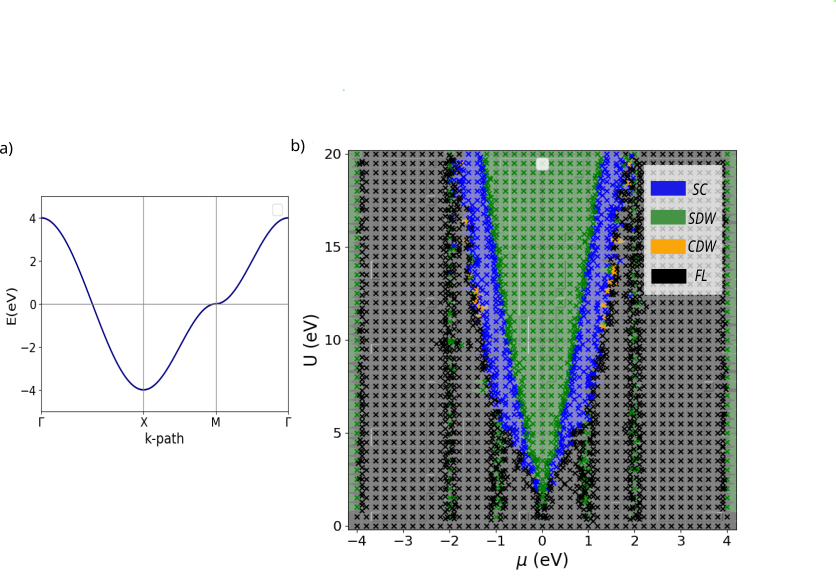
\includegraphics[width=0.95\textwidth]{1NNphased.png}  % Adjust width as needed
    \caption{\textbf{Phase diagram for the 1NN model}:  (t =1eV, nkxnkf = 20x5, ff = 4\AA) as a function of On-site Coulumb Repulsion $U$ and chemical potential $\mu$. 
    Figure shows the four phases observed in the 1NN model: SC (Superconductivity), SDW (Spin-Density Wave), CDW(Charge Density Wave) and FL (Fermu-Liquid).
    Calculated points in the phase diagram are showed by the 'x' markers and a lighter-couloured background is used to depict interpolated regions between these points. }
    \label{fig:1NNpd}
\end{figure}




\subsubsection{Superconductivity in the 1NN Model}

Recent findings have claimed that the 2D Hubbard model does not have a superconducting ground state\cite{qin2020absence}. 
Whilst the model in Ref. \cite{qin2020absence} is the same as the 1NN model explored in this section, their analysis is conducted in a 
slightly different framework than the one used in this project: using DMRG \cite{white1992density} 
at moderate-strong coupling and for values of U between 6-8eV\textit{(which they claim to be the 
regime relevant to the cuprates)}.
The lack of superconductivity in their findings is attributed to a lack of competition 
between the magnetic and superconducting phases. Here, in the weak-coupling framework, both  competition between magnetism and superconductivity and 
a stabilised superconducting region is found. The superconducting order parameter for this stable region is plotted on top of the Fermi-Surface for the first BZ (Fig.\ref{fig:1NNSC}a).
The order parameter shows antisymmetry with respect to a 90 degree rotation and therefore one concludes that
the superconducting region is d-wave symmetric. This is in agreement with what is expected from the Cuprate superconductors \cite{tsuei2000pairing}.\par
\medskip
\noindent 
After plotting the the critical temperature (Tc) as a function of chemical potential ($\mu$) for a constant Coulumb repulsion(U), one observes that
the superconducting critical temperature is maximised closest to the magnetic instability (Fig.\ref{fig:1NNSC}b).
This is in agreement with the idea that competition between instabilities
enhace the phase transition temperature \cite{maple1995interplay,sun2016dome}. Moreover, the magnitude of the Coulumb repulsion and Tc are positively correlated, as is to be expected from the assumed of the pairing mechanism\textit{(See Eq.\ref{Pairing interaction SF})}.
It is important to note that limiting the interactions 
accounted for in the FRG calculation to two-particle interactions acts as a bottle-neck for the accuracy 
of the Tc values calculated. Nevertheless, the trends in Tc remain trustworthy. 

\begin{figure}[htbp]  % Placement: Here, Top, Bottom, Page
    \centering
    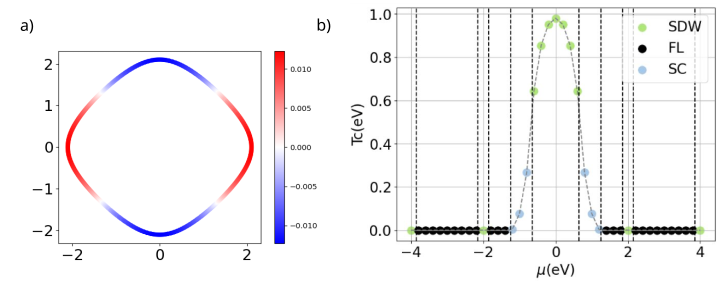
\includegraphics[width=1.0\textwidth]{1NNSC.png}  % Adjust width as needed
    \caption{\textbf{Superconductivity in the 1NN model}:  
    Fig a) Superconducting order parameter projected on Fermi Surface at $\mu$ = 1.00 eV, 
    for U =10.00eV. The order parameter is antisymmetric about a 90 degree rotation and hence
    it exhibits d-wave symmetry. 
    Fig b) Transition temperature (Tc) plotted on a logarithmic scale as a function of chemical potential ($\mu$) for U =10.00eV, showing
    a smooth transition between SC and SDW regions.
    Tc is enhanced closest to the magnetic instability. 
    Although both plots are shown only specific for certain values of U and $\mu$, the results they display hold for the enterity of
    the superconducting region of the phase diagram in Fig.\ref{fig:1NNpd}.  
    }
    \label{fig:1NNSC}
\end{figure}



\subsubsection{Magnetic stripes in the 1NN Model}
\label{subsec:Stripes1NN}

Another distinctive feature of the Cuprates \textit{(as well as other unconventional superconductors}\cite{levi1998stripes}\textit{)} is 
the emergence of "stripes" in their phase diagram. These are patterns of alternating
charge-density and spin density waves\cite{zachar1998landau, vojta2009lattice}. 
In the 1NN model discussed here, these patterns are not observed. However, magnetic regions of 
interest are found outside the main antiferromagnetic (AFM) dome. 
The 1NN phase diagram in Fig.\ref{fig:1NNpd} reveals what will henceforth be referred to as "magnetic stripes" 
occurring at even integer values of the chemical potential ($\mu$). Most of them are ferromagnetically ordered and evolve to some commensurate 
nesting vector as the Coulumb repulsion is increased.\par
\medskip


 
\noindent The physics becomes particularly interesting at a chemical potential of $\mu =1.00eV$. 
In  Cuprates, a dopinf of $\frac{1}{8}$th is known as "the magical doping" \cite{komiya2005magic}, where
stripes emerge and superconductivity is supressed. In this model, the magical doping corresponds 
to a chemical potential of $\pm 1.00eV$(which is $\frac{1}{8}$th of the bandwidth). 
At low Coulumb repulsion values, a ferromagentically ordered spin density wave (SDW) is observed. This SDW is supressed by a superconducting phase,
only to be revived at around $U \approx 15.00eV$, where it becomes antiferromagnetically ordered. The superconducting transition temperature $T_c$ increases along the stripe \textit{(See Fig.\ref{fig:1NN_stripes})}.
While this behaviour is not the same as the convetional stripes seen in cuprates, it is fair to conclude that there is still something 
"magical" about the $\frac{1}{8}$ filling fraction in the 1NN model presented here. \par
\medskip

\noindent It is  worth noting that before conducting this analysis, the possibility of the stripes being a computational artifact was ruled out.
This was done by increasing the $n_k$x$n_{k_f}$ resolution for a single point in the stripe and
confirming that the result remained unchanged. The appearance of these stripes as true outcomes of the calculations is further validated in Section~\ref{subsec:Stripes1NNN}.


\begin{figure}[htbp]  % Placement: Here, Top, Bottom, Page
    \centering
    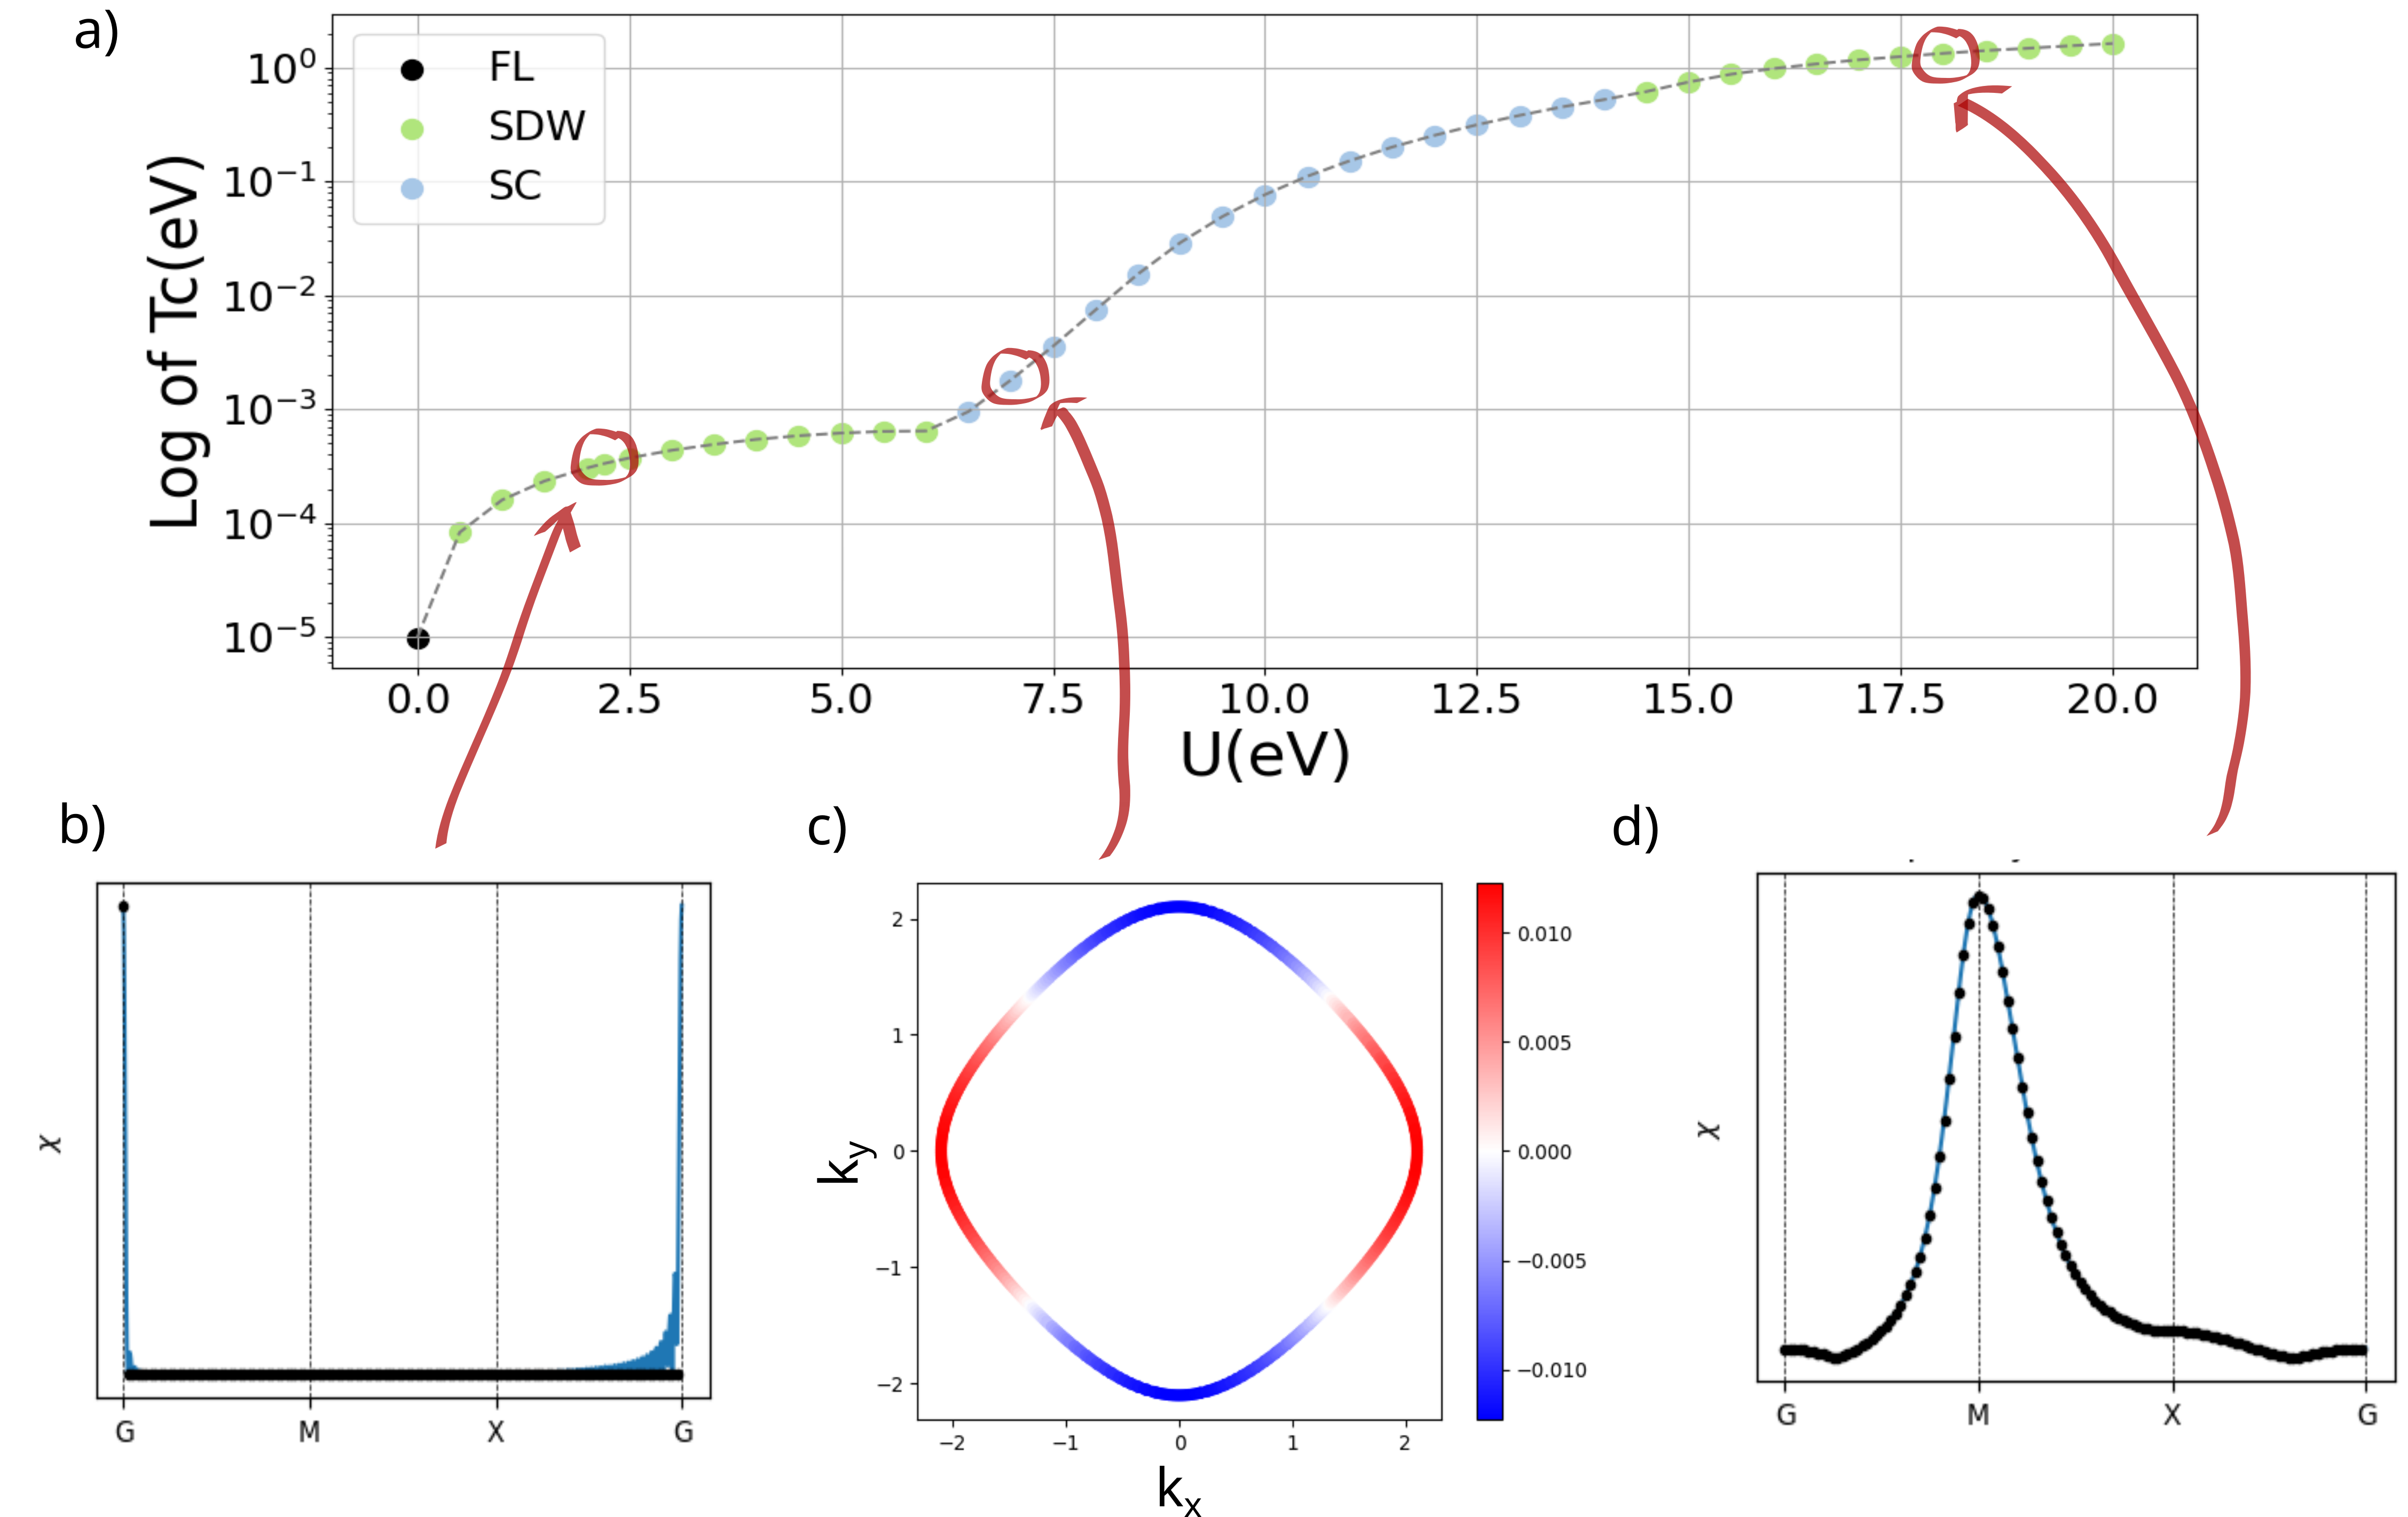
\includegraphics[width=0.9\textwidth]{1NNstripes.png}  % Adjust width as needed
    \caption{\textbf{Magnetic stripe in the 1NN model for doping at $\frac{1}{8}$ of the bandwith}: Fig a) Transition temperature plotted in a Logarithmic scale as a function of Coulumb repulsion (U) along the Magnetic stripe at $\mu$ =1eV. 
       Fig b) Magnetic susceptibility along high symmetry path for U =2.00 eV. 
       Fig c) Plot of the Superconducting order parameter projected on top of the Fermi-surface of the 1NN model for U = 10.00eV and $\mu$ =1.00eV.
       Fig d) Magnetic susceptibility along high symmetry path for U= 18.00eV. Plots showing the susceptibility as a function of \b{q} for both magnetic regions. The Ferromagnetic SDW is supressed by a superconducting phase at U$\approx$ 6.00eV. At larger values of U,  the SDW phase is recovered but with an Anti-Ferromagnetic ordering instead.  }
    \label{fig:1NN_stripes}
\end{figure}



\subsection{Effect of next-nearest neighbour hopping (1NNN model)}
\label{subsec:1NNNModel}
The 1NNN model is an extension of the 1NN model described earlier, incorporating
the next-nearest neighbour hopping amplitude as an additional free parameter.
This section presents three additional phase diagrams
for the two-dimensional Hubbard model, with next-nearest neighbour hopping amplitudes 
of 0.25, 0.50 and 0.75 eV \textit{(See Fig.\ref{fig:1NNN})}.
The nearest neighbour hopping amplitude remains fixed at 1eV for all models. 
Furthermore, the chemical potential of the models is adjusted to ensure a 
constant number of electrons at half-filling, for a direct comparison between the models. \par
\medskip
\noindent
As the next-nearest neighbour hopping is increased, the position of the Van-Hove singularity shifts to lower energies. 
This increase in $t'$ also alters the Fermi-surface, which in turn changes the nesting vectors of the models. 
As a result of both these effects, the SC-SDW-SC sandwich 
region shifts toward the negative chemical potential regime as $t'$ increases.
The superconducting regions remain (in the most-part) d-wave symmetric and the emergence of 
magnetic stripes remains observable. Additionally, general trends in the superconducting transition
temperature ($T_c$) are also observed: it is maximised closest to the 
magnetic instability and it increases as a function of U.\par
\medskip
\noindent Several studies have explored the effect of $t'$ in the 2D Hubbard model, 
employing both FRG \cite{husemann2012incommensurate} and other alternative methods \cite{fontenele2025effects}, 
with a particular focus on using $t'$ as a means to enhance $T_c$. The results presented here take a slightly different approach, aiming to 
compare the features of the 1NN and 1NNN phase diagrams.


\begin{figure}[htbp]  % Placement: Here, Top, Bottom, Page
    \centering
    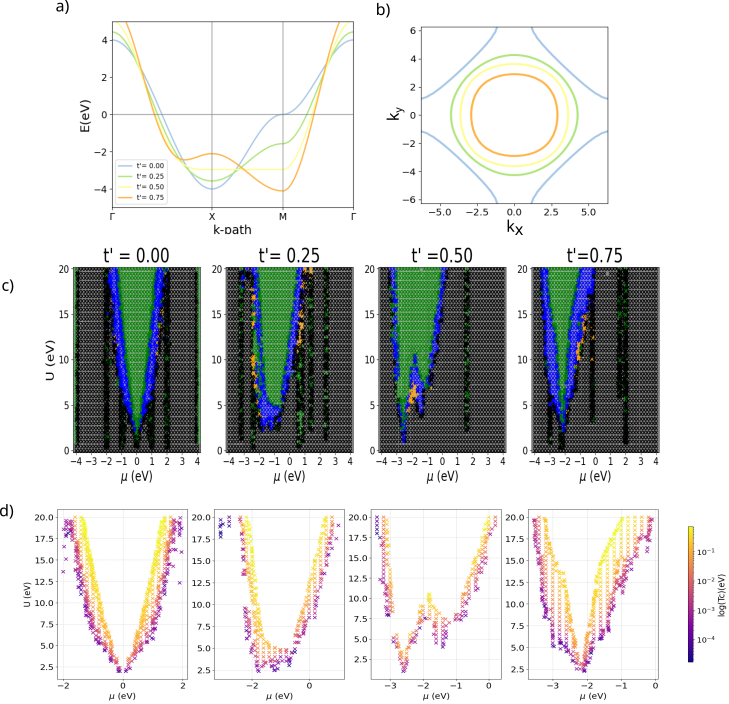
\includegraphics[width=1.0\textwidth]{1NNN.png}  % Adjust width as needed
    \caption{\textbf{1NNN model:}  a) Single plot of the band structure along high-symmetry path for corresponding values of t'.
    b) Single plot of the Fermi surface for all values of t' considered.
    c) Phase diagram for the 1NNN model as a function of Coulumb repulsion U and chemical potential $\mu$ (t =1eV, nkxnkf = 20x5, ff = 4\AA) for t'=0.00, 0.25, 0.50, 0.75 eV. 
    d) Transition temperature for the superconducting region (plotted in a logarithmic scale).
   }
    
    \label{fig:1NNN}
\end{figure}


\subsubsection{Superconductivity in the 1NNN Model}
\label{subsubsec:SC1NNN}

Including a next-nearest neighbour hopping parameter in the 1NN model does not lead to
many significant in the superconducting properties of the model. The order parameter is predominantly d-wave symmetric and the  superconducting temperature ($T_c$) increases
with Coulumb repulsion. Proximity to a Magnetic instability further enhances $T_c$.
Additionally, the same SC-SDW-SC sandwich structure is observed even after breaking particle-hole symmetry, reinfocing the 
idea that that superconductivity is favoured in the vicinity of a  spin density wave (SDW) instability. \par
\medskip
\noindent While most key features remain unchanges, there are some important differences in the superconducting properties. 
When $t' \neq 0 $, charge density wave (CDW) patches appear neighbouring some superconducting regions.
Specifically, when $\frac{t'}{t} = 0.75$, and for Coulumb repulsion between 8 and 11eV, the superconducting order parameter undergoes a change.
Along these horizontal cuts there is a SCI-SDW-SCII-CDW transition. The Superconducting order parameter 
is always d-wave symmetric in the SCI region and for most of the SCII region, but it abruptly transitions to 
s-wave symmetric in the vicinity of the CDW region \textit{(See Fig.\ref{fig:1NNNSC})}. This behaviour is also observed in the SC regions that neighbour CDW regions for 
the $t' = 0.25, 0.50eV$ models. To confirm whether this represents a physical phase transition, one would expect to experimentally observe a 
discontinuity as a result of an additional symmetry breaking when the order parameter shifts from s-wave to d-wave symmetry.

\begin{figure}[htbp]  % Placement: Here, Top, Bottom, Page
    \centering
    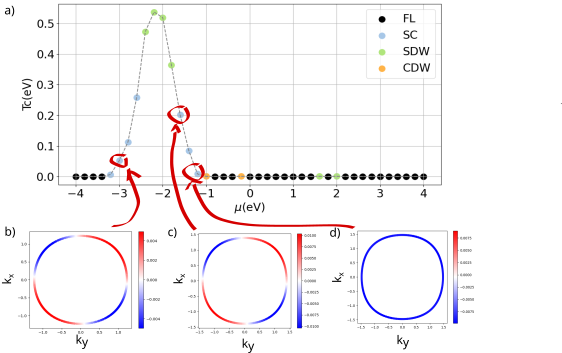
\includegraphics[width=0.90\textwidth]{1NNNSC_075.png}  % Adjust width as needed
    \caption{\textbf{Change in the superconducting order parameter in the t' =0.75eV 1NNN model}: Fig a) Critical temperature plotted in a Logarithmic scale
    as a function of chemical potential $\mu$ for U = 11.50eV.
    The lower panel shows the magnitude of the superconducting order parameter plotted on top of the fermi surface for U= 11.50eV and $\mu$ = -3.0eV, -1.6eV and -1.2eV. These are shown in Figs b)
    c) and d) respectively.  }
    \label{fig:1NNNSC}
\end{figure}



\subsubsection{Magnetic stripes in the 1NNN model}
\label{subsec:Stripes1NNN}

The presence of magnetic stripes is another common feature shared by the 1NN and 1NNN models, 
further supporting its physical origin.
A summary of all the stripes and their respective nesting vectors is provided 
in Table.\ref{tab:StripesSummary}. The locations of these
stripes suggest that their formation is a consequence of strong nesting at specific 
chemical potential values. 
Notably, the stripe at "magic doping" is the only to undergo a change ordering from ferromagnetic (FM) 
to antiferromagnetic (AFM) as a result of the strong competition with Superconductivity. 



\medskip 

\noindent While the transition from a Fermi liquid phase to any of the superconducting (SC), spin density wave (SDW), or charge density wave (CDW) phases is quite abrupt, the critical temperature
evolves more smoothly for stripes where there is a strong competition between SC and SDW/CDW instabilities \textit{(see Fig.\ref{fig:1NNNStripes})}. 
This is consistent with the discussion in Section \ref{subsec:Stripes1NN}. When $\frac{t'}{t} = 0.50$, a magnetic double dome emerges, becoming more pronounced as the Coulomb repulsion increases \textit{(see Fig.\ref{fig:1NNNDome})}. 
This is the pattern one might expect in the superconducting region, as observed in cuprates \cite{taillefer2010scattering}. 
However, this trend is only observed in this particular model and phase.



\begin{table}[h]
    \centering
    \begin{tabular}{|c|c|c|c|c|c|c|}
        \hline
       t'(eV) & $\mu$ (eV) & Competing with other phase?& Nesting vector & Magnetic ordering  \\
        \hline
        0.00 & 1.00 & Yes (SC) & (0,0)-($\pi$, $\pi$)& FM-AFM\\
        \hline
        0.00 & 2.00 &  No  & (0,0)-(0, $\pi$)  & FM-Commensurate\\
        \hline
        0.25 & -3.20 & No  & (0,0)  & FM\\
        \hline
        0.25 & -2.40 & No  & (0,0) & FM\\
        \hline
        0.25 & -2.00 & No  & (0,0)-($\pi$, $\pi$)  & FM - AFM\\
        \hline
        0.25 & 0.60 &  No  & (0,0)  & FM \\
        \hline
        0.25 & 1.40 &  Yes (CDW)  & (0,0)  & FM \\
        \hline
        0.25 & 2.40 &  No  & (0,0)  & FM \\
        \hline
        0.50 & -2.60 &  No  & (0,0)  & FM \\
        \hline
        0.50 & 1.60 &  No  & (0,0)  & FM \\
        \hline
        0.75 & -3.00 &  Yes(SC)  & (0,0)  & FM \\
        \hline
        0.75 & -2.20 &  Yes(SC)  & (0,0)-inc. & FM- Incommensurate \\
        \hline
        0.75 & 2.00 &  No  & (0,0). & FM \\
        \hline


          
        \hline
    \end{tabular}
    \caption{\textbf{Survey of stripes in the 1NNN model.} Table summarising the location and magnetic ordering of the Stripes in the 1NNN model .}
    \label{tab:StripesSummary}
\end{table}

\begin{figure}[htbp]  % Placement: Here, Top, Bottom, Page
    \centering
    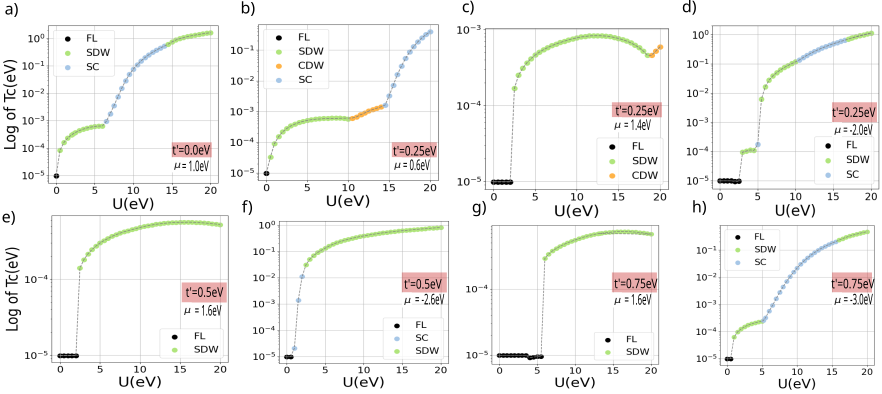
\includegraphics[width=0.90\textwidth]{1NNNstripes.png}  % Adjust width as needed
    \caption{\textbf{Tc as a function of Coulumb repulsion for a selection of stripes in the 1NNN model}: Tc plotted in
    a logarithmic scale for stripes at:  Fig a) t' = 0.00eV, $\mu$=1.00eV, b) t' = 0.25eV, $\mu$=0.60eV, c) t' = 0.25eV, $\mu$=1.40eV,
    d) t' = 0.25eV, $\mu$=-2.00eV,
    e) t' = 0.50eV, $\mu$=1.60eV,
    f) t' = 0.50eV, $\mu$=-2.60eV,
    g) t' = 0.75eV, $\mu$=1.60eV, 
    h) t' = 0.75eV, $\mu$=-3.00eV.}
    \label{fig:1NNNStripes}
\end{figure}

\noindent
\begin{minipage}[t]{0.48\textwidth}
    \centering
    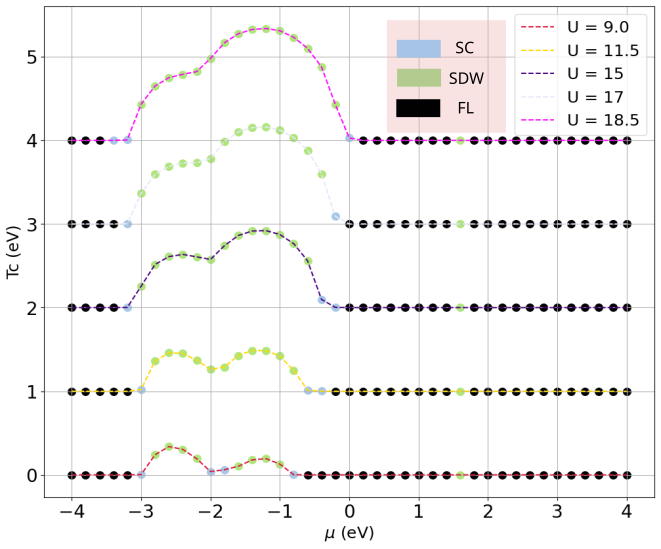
\includegraphics[width=\textwidth]{1NNN050Dome.png}
    \captionof{figure}{\textbf{Magnetic Dome in 1NNN, t'=0.50eV model}: Tc as a function of $\mu$ for different values of U (offsetted by 1eV).
    This figure shows how the height of the second magentic dome increases as a function of U whilst the height of the 
    first remains constant. The turning point of the double dome pattern occurs at $\mu$=-2.00eV }
    \label{fig:1NNNDome}
\end{minipage}
\hfill
% Second figure (right side)
\begin{minipage}[t]{0.48\textwidth}
    \centering
    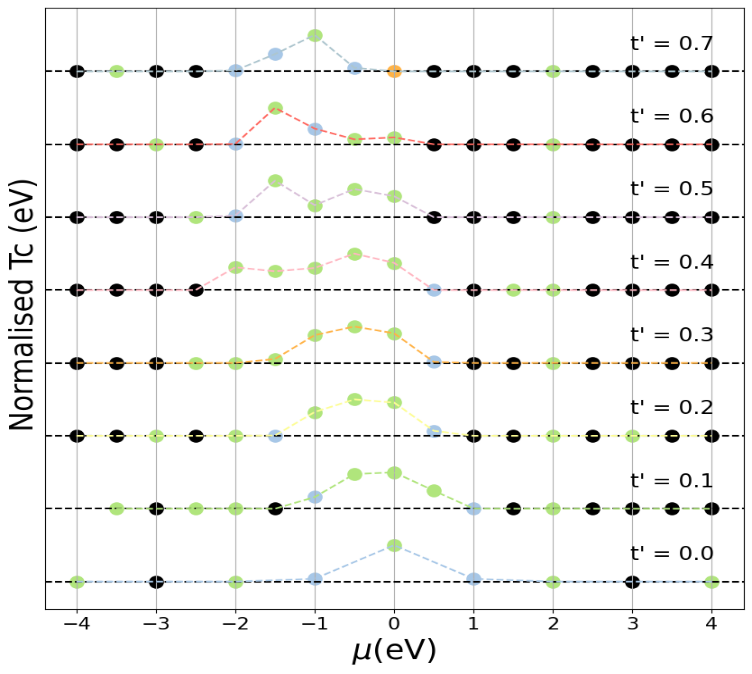
\includegraphics[width=\textwidth]{tprimecont.png}
    \captionof{figure}{\textbf{Continuous variation of t':} Normalised Tc plotted as a function of chemical 
    potential $\mu$ for several values of t'. Tc is normalised separatedly with respect to the 
    maxima of each plot in order to allow for the clear vizualisation of the trend.  }
    \label{fig:tprimecont}
\end{minipage}



\subsubsection{Continous variation of next-nearest neighbour hopping}

In order to support further the ideas discussed in Section \ref{subsec:1NNModel}, the critical temperature
is plotted as a function of chemical potential $\mu$ for different values of t' at U=10.00eV \textit{(See Fig.\ref{fig:tprimecont})}
One can see how the Magnetic region is pushed to more negative values of the chemical potential as the value of the next-nearest 
neighbour hoping parameter is increased (and the van Hove singularity is pushed down in energy). The bulk magnetic
region remains AFM ordered and the SC order parameter is in most cases d-wave symmetric. The exception to this is the case where
t' is set to 0.70eV. There, the SC order parameter transitions to s-wave symmetric when it is closest to the boundary 
with the CDW phase (as discussed in Section \ref{subsubsec:SC1NNN}).

\subsection{Effect of bi-orbital system (1NN2 model)}
\label{subsec:1NN2Model}

The models presented so far were constructed assuming a single orbital per site. This section discusses the effect of including
two orbitals per site. The model was calculated using the parameters discussed in Section \ref{subsec:TBM1NN2} and since it now includes
multiple orbitals per site its Hamiltonian is now extended to the Hubbard-Kanamori Hamiltonian \textit{(See Section \ref{subsubsec: HKmodel})}. 
The chemical potential is fixed to the undoped ($\mu = 0.00eV $) and doped ($\mu =1.00eV$). The Coulumb repulsion and Hunds coupling strengths are varied from 1-10eV and 0.1-1.0eV respectively.
The points were calculated using a form factor of 4\AA and an $n_k$x$n_{k_f}$ grid of 20x5. 
First, this section will focus on the 1NN2MY model, where the orbital mixing between different orbitals is set to 0. This is later compared
to the 1NN2MN where this orbital mixing is included in the model. \par
\medskip
\noindent In the undoped case, the model shows an Antiferromagnetically ordered SDW ground state
for $U > 3.00eV$. The groundstate transitions to a CDW if the Coulomb repulsion is set to 0. This CDW region has a nesting vector 
of $(\pi, \pi)$. Doping the system to a chemical potential of $\mu = 1.00eV$ supresses the SDW. Instead, a small superconducting patch 
emerges in the boundary of a CDW phase \textit{(See Fig.{\ref{fig:1NN2pd}})}. The magnitude of the Hund's coupling plays a small role in the dominating phase of the Tc of the model. The Superconducting regions shown in Fig.\ref{fig:1NN2pd}d. show different order parameters. The SC region at U=0.0eV is s-wave symmetric whilst the SC region at U =10.00eV
is d-wave symmetric. Comparing figures \ref{fig:1NN2pd}c,d with e,f allow one to conclude that the inclusion of
different orbital hopping favours the emergence of a CDW phase for lower Coulumb repulsion values in the doped to $\mu = 1.00eV$ case. 

\begin{figure}[htbp]  % Placement: Here, Top, Bottom, Page
    \centering
    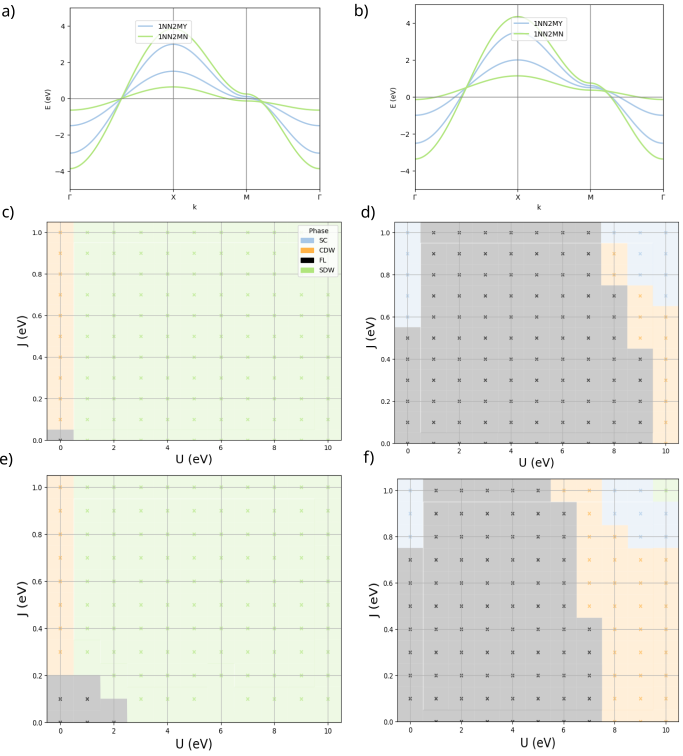
\includegraphics[width=0.90\textwidth]{1NN2.png}  % Adjust width as needed
    \caption{\textbf{Phase diagram for the 1NN2 model:} Phase diagram for the 1NN2 model without orbital 
    mixing between different orbitals. Fig a) Band structure for the undoped 1NN2MY/N model. 
    Fig b) Band structure for the 1NN2MY/N model at $\mu =1.0eV$. 
    Fig c) Phase diagram for the undoped 1NN2MY model.
    Fig d) Phase diagram for the 1NN2MY model at $\mu =1.00eV$.
    Fig e) Phase diagram for the undoped 1NN2MN model.
    Fig f) Phase diagram for the 1NN2MN model at $\mu =1.00eV$.}
    \label{fig:1NN2pd}
\end{figure}
\newpage
\section{Conclusion and Outlook}

This project aimed to investigate the interplay between Magnetism and Superconductivity in the 2D Hubbard Model at half-filling. The calculations were carried out
in the spin-fluctuation mediated superconductivity framework using the two-particle truncated TU$^2$FRG scheme in the weak-coupling limit. Whilst this method
fails to capture correlated phases such as Mott-instulating or pseudo-gap phases, it is widely in agreement with previous literature. The results presented here provide
a comprehensive study of this model for a uniquely wide range of parameters. A strong competition between an
Antiferromagnetically-ordered SDW and d-wave symmetric SC phase is observed. Moreover, several routes to stabilise and enhance the critical 
temperature of the Superconductor are found: to increase the magnitude of the On-site Coulumb repulsion and to be in the vicinity of a stabilised SDW region. 
Narrow magnetic stripes are present and their ordering is found to change at the "magical doping" value. The effect of including a next-nearest neighbour hopping parameter 
is studied in depth. Increasing t' pushes the Van Hove singularity towards more negative energy values, resulting in an overall
shift of the region where the interplay between SDW and SC is most prominent towards more negative chemical potential values. A Magnetic double dome emerges for a ratio of $\frac{t'}{t} = 0.50$.
The inclusion of a next-nearest neighbour hopping parameter gives rise to stable CDW patches surrounding the SC regions. The SC order parameter
transitions from d-wave to s-wave symmetric in the vicinity of such patches. Finally, a preliminary analysis is conducted on the effect of
extending such models to the two-orbital per site case. The AFM ground state is supressed as a function of dopping and the magnitude of the Hund's coupling
plays little role on the phases observed.\par
\medskip

\noindent Future work could include a deeper analysis of the two-orbital per site model. This could include exploring wider ranges of chemical potential and Hund's coupling values. Moreover, it
would be very interesting to extend this further to the case of a bi-layer two-orbital per site Hubbard model. 
One could then also look at how Spin-orbit coupling (SOC) affects the results obtained. It can quite quickly escalate to a multi-dimensional analysis and there are many avenues to explore. 
However, one of great interest and relevance would be to continue
to, step-by-step, increase the complexity of these models to eventually resemble that of some unconventional superconductors such as Lanthium Nickelate, focusing on how the different steps
affect the interplay between magentism and superconductivity. This would mean that one has, starting from the findings presented here, 
a step-by-step analysis of how the Tc and superconducting region of a more complex model change with model parameters. All of which could serve
as a route towards understanding what key parameters play a role in the superconducting phases of unconventional superconductors. 






\newpage

\bibliographystyle{unsrt}  % Choose a style such as plain, alpha, abbrv, etc.
\bibliography{references}

\end{document}